%%%%%%%%%%%% STRUCTURE %%%%%%%%%%%%%%%
\documentclass[a4paper,12pt]{article}
\usepackage[T1]{fontenc}
\usepackage[utf8]{inputenc}
\usepackage[brazil]{babel}
\usepackage{lmodern}
\usepackage{setspace}
\usepackage[top=2cm, bottom=2cm, left=2cm, right=2cm]{geometry}
\usepackage{listings}
\usepackage{xcolor}
\usepackage{amsmath}
\usepackage{ragged2e}

\lstset{
    basicstyle=\ttfamily\small,
    keywordstyle=\color{blue}\bfseries,
    stringstyle=\color{red},
    commentstyle=\color{gray}\itshape,
    numbers=left,
    numberstyle=\tiny\color{gray},
    stepnumber=1,
    numbersep=8pt,
    backgroundcolor=\color{white},
    showspaces=false,
    showstringspaces=false,
    showtabs=false,
    frame=single,
    rulecolor=\color{black!20},
    tabsize=4,
    captionpos=b,
    breaklines=true,
    breakatwhitespace=false,
}
%%%%%%%%%%%%%%%%%%%%%%%%%%%%%%%%%%%%%%

%%%%%%%%%%%%%%%% PAGES STYLE %%%%%%%%%
\usepackage{fancyhdr}
\fancypagestyle{main}{
\renewcommand{\headrulewidth}{0pt}
\fancyhead[RO]{\thepage}
\fancyfoot[CO]{}
}
%%%%%%%%%%%%%%%%%%%%%%%%%%%%%%%%%%%%%%

\usepackage{graphicx}
\usepackage{epstopdf}
\usepackage{subfig}
\usepackage{mathptmx}
\usepackage{changepage}
%\usepackage[alf]{abntex2cite}

%%%%%%%%%%% PDF METADATA %%%%%%%%%%%%%
\usepackage[ pdftitle={MODELO RELATÓRIO},
pdfsubject={INTRODUÇÃO AO LABORATÓRIO DE CONTROLE - Grupo 3},
pdfkeywords={Controle,Automação,UFRN,DCA,ipump},
hidelinks]{hyperref}
%%%%%%%%%%%%%%%%%%%%%%%%%%%%%%%%%%%%%%

\begin{document}

\onehalfspacing

\thispagestyle{empty}

\setcounter{page}{1}

%%%%%%%%%%%% LOGOS %%%%%%%%%%%%%%%%%%%

\begin{figure}[!ht]

\centering

\subfloat{

\includegraphics[width=2.7cm]{UFRN.eps}
\label{UFRN Logo}
}
\hspace{11.09cm}
\subfloat{

\includegraphics[width=2.4cm]{DCA.eps}
\label{DCA Logo}
}

%\caption{}
\label{Logos}

\end{figure}

%%%%%%%%%%%%%%% CAPA %%%%%%%%%%%%%%%%%

\vspace{-1cm}

\begin{center}
{\bf{\normalsize UNIVERSIDADE FEDERAL DO RIO GRANDE DO NORTE\\
CENTRO DE TECNOLOGIA\\
DEPARTAMENTO DE ENGENHARIA DE COMPUTAÇÃO E AUTOMAÇÃO\\
ENGENHARIA DE COMPUTAÇÃO E ENGENHARIA MECATRÔNICA
}}


\vspace{3.6cm}

{\bf{\large RELATÓRIO DA 1º EXPERIÊNCIA\\ % Pensar em como dividir entre os experimentos
LEVANTAMENTO DA CURVA DO SENSOR\\
}}
\vspace{1.5cm}
{\large TURMA: 1\\
	GRUPO 20262G4T1}

\vspace{3.6cm}



\begin{flushright}
\begin{normalsize}
Danilo Isamu Pereira Hikague: 20230072008\\
\vspace{0.8cm}
Murilo de Lima Barros: 20250070735\\
\vspace{0.8cm}
Rafael Cabral Melo: 20210080441\\
\vspace{0.8cm}
Ramon Vinicius Ferreira de Souza: 20220017441\\
\vspace{0.8cm}
Virna Emanuelle Veloso Aguiar:: 20220025354\\ 
\end{normalsize}
\end{flushright}


\vspace{2.5cm}

{\large Natal-RN\\
2026}

\end{center}

\newpage

%%%%%%%%%%%%%%%  CONTRA-CAPA %%%%%%%%%

\thispagestyle{empty}

\begin{center}
\begin{normalsize}
NOME COMPLETO 1º ALUNO: Nº MATRÍCULA\\
\vspace{0.8cm}
NOME COMPLETO 2º ALUNO: Nº MATRÍCULA\\
\vspace{0.8cm}
NOME COMPLETO 3º ALUNO: Nº MATRÍCULA\\
\vspace{0.8cm}
NOME COMPLETO 4º ALUNO: Nº MATRÍCULA\\

\end{normalsize}
\end{center}
\vspace{3cm}

{\bf{\large {\centering TÍTULO DA EXPERIÊNCIA\\}}}

\vspace{4cm}

\begin{adjustwidth}{7.5cm}{0cm}

{\normalsize

Primeiro Relatório Parcial apresentado à disciplina de
Projeto de Sistemas de Controle - Laboratório, correspondente à
avaliação da 1º unidade do semestre 2026.2 do 7º período
dos cursos: Engenharia de Computação e Engenharia Mecatrônica da
Universidade Federal do Rio Grande do Norte, sob
orientação do {\bf Prof. Fábio Meneghetti Ugulino de
Araújo.}

}

\end{adjustwidth}

\vspace{2cm}

\begin{center}

Professor:  Fábio Meneghetti Ugulino de Araújo.

\vspace{2.5cm}

{\large Natal-RN\\
2026}

\end{center}

\newpage

%%%%%%%%%%%%%%%  RESUMO %%%%%%%%%%%%%%

\thispagestyle{empty}

\begin{center}
{\large \textbf{RESUMO}}
\end{center}

\vspace{3cm}

\begin{justify}

\hspace{4ex}Trata-se da apresentação fiel, breve e concisa dos aspectos mais relevantes do
trabalho, apresentando as ideias essenciais, na mesma progressão e no mesmo
encadeamento que aparecem no texto. O resumo deve apresentar os objetivos, uma
visão geral, ampla e, ao mesmo tempo, clara e objetiva do conteúdo do trabalho.\\
\hspace{4ex}A norma da ABNT recomenda que se use de 150 a 500 palavras, em espaço
simples, e deve-se usar o verbo na voz ativa e na terceira pessoa singular. Logo abaixo,
devem ser colocadas as palavras-chave.\\

\end{justify}

\vspace{1.5cm}

\textbf{Palavras-chave:}

\newpage

%%%%%%%%%%%%%%%  LISTA DE SÍMBOLOS %%%

\thispagestyle{empty}

\begin{center}
{\large \textbf{LISTA DE SÍMBOLOS}}
\end{center}

\vspace{3cm}

\begin{tabular}{ l l }
A\hspace{1.5cm} & Matriz triangular superior com diagonal unitária.\\
\phantom{a} & \phantom{a}\\
D\hspace{1.5cm} & Matriz diagonal obtida a partir de $W^{T}W$\\
\phantom{a} & \phantom{a}\\
$\theta$\hspace{1.5cm} & Vetor de parâmetros.\\
\phantom{a} & \phantom{a}\\
$\Xi$\hspace{1.5cm} & Vetor de resíduos de modelagem.\\
\phantom{a} & \phantom{a}\\
d\hspace{1.5cm} & Tempo de retardo de um sistema ou tempo morto.\\
\phantom{a} & \phantom{a}\\
e(k)\hspace{1.5cm} & Resíduo (Erro de Estimação mais o Ruído).\\
\end{tabular}

\newpage

%%%% LISTA DE ABREVIATURAS E SIGLAS %%

\thispagestyle{empty}

\begin{center}
{\large \textbf{LISTA DE ABREVIATURAS E SIGLAS}}
\end{center}

\vspace{3cm}

\begin{tabular}{ l l }
ARX\hspace{1.5cm} & Matriz triangular superior com diagonal unitária.\\
ARMAX\hspace{1.5cm} & Matriz diagonal obtida a partir de $W^{T}W$\\
NARX\hspace{1.5cm}&Vetor de parâmetros.\\
NARMAX\hspace{1.5cm}&Vetor de resíduos de modelagem.\\
MQ\hspace{1.5cm}&Tempo de retardo de um sistema ou tempo morto.\\
\end{tabular}

\newpage

%%%%%%%%% LISTA DE FIGURAS %%%%%%%%%%%

\thispagestyle{empty}

\begin{center}
\listoffigures
\end{center}

\newpage

%%%%%%%%%%%%%%% SUMÁRIO %%%%%%%%%%%%%%

\thispagestyle{empty}

\begin{center}
\tableofcontents
\end{center}

\newpage

%%%%%%%%%%%%%%% INTRODUÇÃO %%%%%%%%%%%

\thispagestyle{main}

\section{INTRODUÇÃO}

\begin{justify}
\hspace{4ex}A obtenção de modelos matemáticos quantitativos constitui uma etapa fundamental na solução e na análise de problemas de controle, sendo um requisito para que um sistema físico atenda a especificações de desempenho determinadas anteriormente. Para atuar corretamente sobre a dinâmica de uma planta, o sistema de controle deve ser capaz de interpretar as grandezas físicas envolvidas com precisão. Neste contexto, este relatório documenta a obtenção da curva de resposta do sensor de nível para um sistema de tanques acoplados da Quanser\textregistered.
\end{justify}

\begin{justify}
\hspace{4ex}O sistema didático utilizado é composto por um reservatório, uma bomba, tubos flexíveis e dois tanques. Cada tanque é dotado de um sensor de nível que fornece um sinal elétrico de tensão proporcional à altura da coluna de líquido. O objetivo deste experimento é estabelecer a relação matemática direta entre a grandeza física medida (nível da água em centímetros) e o sinal elétrico lido pelo sistema de aquisição (tensão em \textit{volts}), calibração esta que é indispensável para as futuras estratégias de controle de nível.
\end{justify}

\newpage

%%%%%%%%%% REFERENCIAL TEÓRICO %%%%%%%

\thispagestyle{main}

\section{REFERENCIAL TEÓRICO} % Pendente (se formos fazer)

Trata-se da apresentação do embasamento teórico sobre o qual se fundamentará
o trabalho, ou seja, são os pressupostos que darão suporte à abordagem do trabalho.
Lembrar de sempre que utilizar texto de outros lugares, utilizar citação da fonte, como por exemplo, \cite{LATEX04}.

\subsection{Seções}

\subsubsection{Subseções}

\newpage

%%%%%%%%%% METODOLOGIA %%%%%%%%%%%%%%%

\thispagestyle{main}

\section{METODOLOGIA}

\begin{justify}
    \hspace{4ex}O experimento foi conduzido utilizando a bancada do sistema de tanques acoplados da Quanser\textregistered. O aparato físico foi integrado a um microcomputador operando com Windows, munido dos softwares MATLAB\textregistered/SIMULINK\textregistered  e QUARC\textregistered, que formam o ambiente de simulação e controle. O interfaceamento entre a planta física e o microcomputador foi realizado por meio de uma placa de aquisição de dados Q8-USB e do módulo de potência VoltPAQ-X1\textregistered.
\end{justify}

\begin{justify}
    \hspace{4ex}A prática, designada como experimento 1.B., consistiu no levantamento de dados estáticos para a modelagem do sensor de nível. O procedimento foi executado estabelecendo-se diferentes volumes de líquido no tanque 1, de forma a registrar a tensão elétrica fornecida pelo sensor em cinco alturas pré-determinadas: 5, 10, 15, 20 e 25 cm.
\end{justify}

\begin{justify}
    \hspace{4ex}Para garantir a confiabilidade dos dados e mitigar ruídos ou variações pontuais, o roteiro estipula a realização de múltiplos ensaios para um mesmo ponto de operação. Ao todo, foram realizadas 6 baterias de medições para cada patamar de nível. A partir dos dados obtidos relacionando a altura da coluna de água ($h$) e a tensão lida ($u$), a curva estática do sensor foi ajustada computacionalmente utilizando a linguagem Python, aplicando o método de regressão linear por mínimos quadrados através da função \texttt{numpy.polyfit}.
\end{justify}

\begin{justify}
    \hspace{4ex}O algoritmo desenvolvido para o processamento das leituras, estimação dos parâmetros $a$ e $b$ da equação da reta ($h = au + b$) e geração do gráfico de dispersão com o modelo ajustado é apresentado no Código~\ref{lst:regressao_python}.
\end{justify}

\begin{lstlisting}[language=Python, caption={Algoritmo em Python para regressão linear por mínimos quadrados e geração do gráfico.}, label={lst:regressao_python}]
import numpy as np
import matplotlib.pyplot as plt
from pathlib import Path

def estimate_function(h_values, u_read):
    """
    Estima os coeficientes a e b da reta h = a*u + b usando minimos quadrados.
    """
    h_all = []
    u_all = []
    
    for value in u_read:
        u_all.extend(value)
        h_all.extend(h_values)
        
    u_all = np.array(u_all)
    h_all = np.array(h_all)
    
    coefs = np.polyfit(u_all, h_all, 1)
    a, b = coefs
    
    return a, b, u_all, h_all

def plot_regression(a, b, u_all, h_all):
    """
    Gera o grafico de dispersao com a reta de regressao plotada.
    """
    u_line = np.linspace(min(u_all)*0.9, max(u_all)*1.1, 100)
    h_line = a * u_line + b
    output = Path('outputs/1b.png')
    
    plt.figure(figsize=(8, 6))
    plt.scatter(u_all, h_all, color='blue', label='Dados Coletados (h vs u)', zorder=5)
    plt.plot(u_line, h_line, color='red', linestyle='--', label=f'Reta Ajustada: $h = {a:.3f}u {b:+.3f}$')
    
    plt.title('Regressao Linear: Altura do Tanque (h) vs Sinal de Tensao (u)')
    plt.xlabel('u (V)')
    plt.ylabel('h (cm)')
    plt.legend()
    plt.grid(True, linestyle='--', alpha=0.7)
    plt.savefig(output)
    print(f"\n Arquivo salvo em {output}")

if __name__ == "__main__":
    h = [5, 10, 15, 20, 25]
    
    u_read = [
        # Dados
    ]
    
    a, b, u_all, h_all = estimate_function(h, u_read)
    
    print("-" * 40)
    print(f"a: {a:.4f}")
    print(f"b: {b:.4f}")
    print(f"h = {a:.4f} * u {b:+.4f}")
    print("-" * 40)
    
    plot_regression(a=a, b=b, u_all=u_all, h_all=h_all)
\end{lstlisting}


\subsection{Seções}

\subsubsection{Subseções}

\newpage

%%%%%%%%%% RESULTADOS %%%%%%%%%%%%%%%

\thispagestyle{main}

\section{RESULTADOS}

\begin{justify}
    \hspace{4ex}Os valores de tensão obtidos nas 6 medições para os cinco valores de altura da coluna de água ($h = 5, 10, 15, 20, 25\text{ cm}$) estão consolidados na Tabela~\ref{tab:dados_laboratorio}, acompanhados das respectivas médias aritméticas calculadas para cada ponto estático.
\end{justify}

\begin{table}[htbp]
\centering
\caption{Tensão lida no sensor de nível em função da altura da coluna de líquido.}
\label{tab:dados_laboratorio}
\begin{tabular}{|c|c|c|c|c|c|c|c|}
\hline
\textbf{\begin{tabular}[c]{@{}c@{}}Altura $h$\\ (cm)\end{tabular}} & 
\textbf{\begin{tabular}[c]{@{}c@{}}Med. 1\\ (V)\end{tabular}} & 
\textbf{\begin{tabular}[c]{@{}c@{}}Med. 2\\ (V)\end{tabular}} & 
\textbf{\begin{tabular}[c]{@{}c@{}}Med. 3\\ (V)\end{tabular}} & 
\textbf{\begin{tabular}[c]{@{}c@{}}Med. 4\\ (V)\end{tabular}} & 
\textbf{\begin{tabular}[c]{@{}c@{}}Med. 5\\ (V)\end{tabular}} & 
\textbf{\begin{tabular}[c]{@{}c@{}}Med. 6\\ (V)\end{tabular}} & 
\textbf{\begin{tabular}[c]{@{}c@{}}Média\\ (V)\end{tabular}} \\ \hline
5  & 0,692 & 0,763 & 0,761 & 0,783 & 0,775 & 0,776 & 0,7583 \\ \hline
10 & 1,546 & 1,548 & 1,544 & 1,595 & 1,565 & 1,556 & 1,5590 \\ \hline
15 & 2,336 & 2,363 & 2,345 & 2,416 & 2,359 & 2,372 & 2,3652 \\ \hline
20 & 3,173 & 3,155 & 3,131 & 3,175 & 3,176 & 3,212 & 3,1703 \\ \hline
25 & 3,931 & 3,957 & 3,915 & 3,911 & 3,925 & 3,921 & 3,9267 \\ \hline
\end{tabular}
\end{table}

\begin{justify}
    \hspace{4ex}Submetendo o conjunto integral de 30 pontos amostrais ao método dos mínimos quadrados usando o algoritmo implementado, foram determinados os coeficientes angular ($a$) e linear ($b$), obtendo-se a relação:
\end{justify}

\begin{equation}
    h = 6{,}287 \, u + 0{,}188
    \label{eq:reta_calibracao}
\end{equation}

\begin{justify}
    \hspace{4ex}A Figura~\ref{fig:curva_calibracao} ilustra os pontos experimentais sobrepostos à reta de regressão ajustada.
\end{justify}

\begin{figure}[htbp]
    \centering
    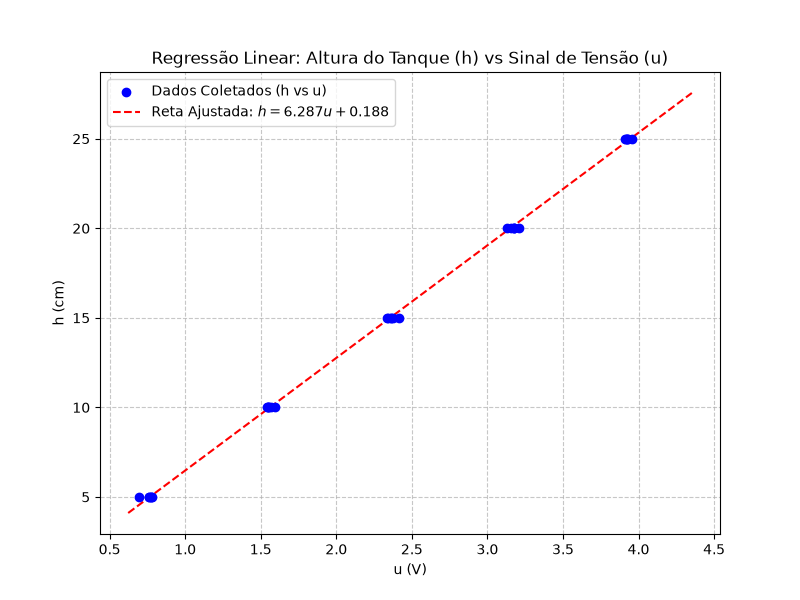
\includegraphics[width=0.75\textwidth]{img/1b.png}
    \caption{Curva estática do sensor de nível com dispersão dos pontos e reta ajustada por mínimos quadrados.}
    \label{fig:curva_calibracao}
\end{figure}

\begin{justify}
    \hspace{4ex}Observa-se um comportamento estritamente linear em toda a faixa operacional avaliada (\text{de }$5\text{ a }25\text{ cm}$). O coeficiente de sensibilidade obtido ($a \approx 6{,}287\text{ cm/V}$) demonstra excelente concordância com o valor de calibração de referência teórico da planta ($6{,}25\text{ cm/V}$), apresentando uma diferença de cerca de 1\%. O pequeno coeficiente linear positivo ($b \approx 0{,}188\text{ cm}$) reflete a variação residual de tensão na medição do zero ou variações no referencial do fundo do tanque.
\end{justify}

\newpage

%%%%%%%%%% CONCLUSÃO %%%%%%%%%%%%%%%

\thispagestyle{main}

\section{CONCLUSÃO}


\hspace{4ex}A conclusão, além de guardar uma proporção relativa ao tamanho do trabalho,
deve guardar uma proporcionalidade também quanto ao conteúdo. Não deve conter
assuntos desnecessários, nem exageros numa linguagem excessivamente técnica e
rebuscada. A conclusão deve dar respostas às questões do trabalho, correspondente aos
objetivos propostos. Deve ser breve, podendo, se necessário, apresentar sugestões para
pesquisas futuras.

\newpage

%%%%%%%% REFERÊNCIAS %%%%%%%%%%%%%%%%%

% Referências bibliogáficas (geradas automaticamente)
\addcontentsline{toc}{chapter}{Referências bibliográficas}
\bibliography{bib/bibliografia}

\appendix

%Apêndice A
\include{apendice}

\end{document}
